\documentclass{article}
\usepackage[light, inline-math]{chs-physics-report}
\usepackage{float}
\usepackage{pgfplots}
\usepackage{pgfplotstable}
\usepackage{booktabs}

\pgfplotsset{compat=1.18}

\title{5.3: Static Equilibrium Labs}
\name{Gavin Chen}
\ww{Cole TerBush and Tim Marijono}

\begin{document}
\section{Lab 1}
\section*{Objective}
To find the tension force required to hold up a ruler with a hanging mass.
\section*{Diagram}
\begin{figure}[H]
    \centering
    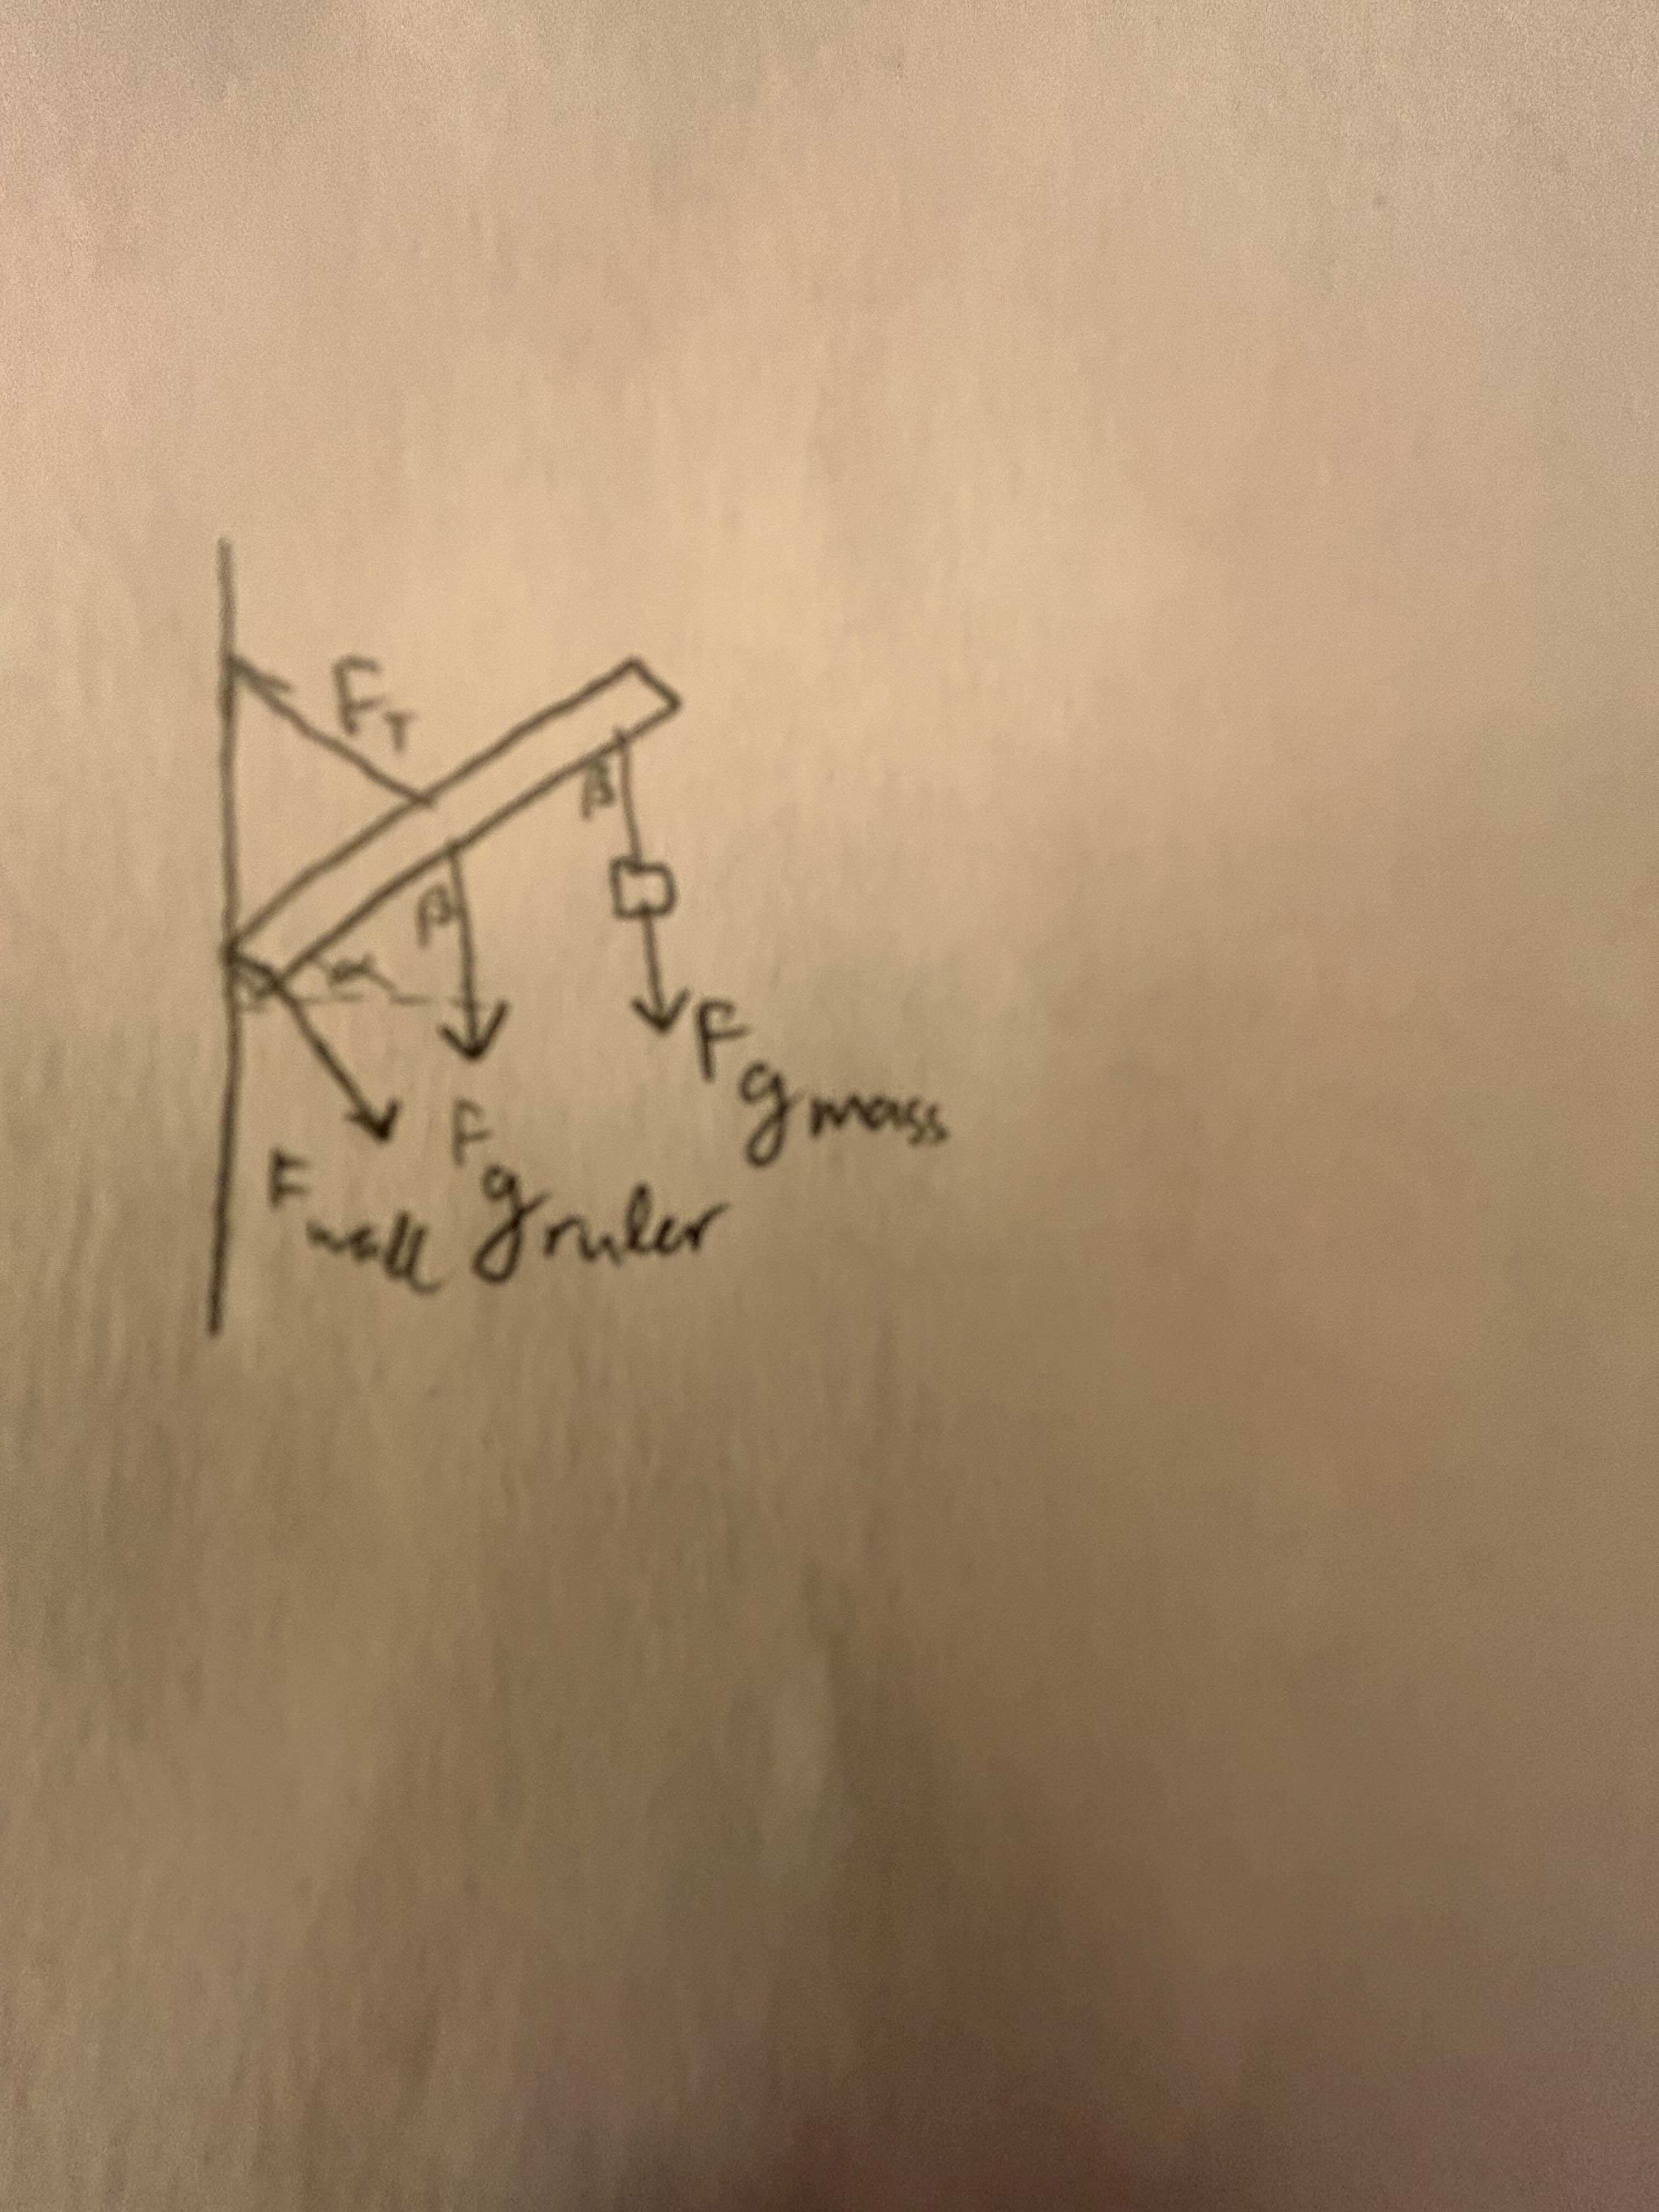
\includegraphics[height=15cm]{Lab 5.3.1.jpg}
\end{figure}
\section*{Derivation}
\[\tau = F_Tr_{string}\sin(\alpha) - {F_g}_{ruler}r_{ruler}\sin(\beta) - {F_g}_{mass}r_{mass}\sin(\beta)\]
\[F_T = \frac{\tau + {F_g}_{ruler}r_{ruler}\sin(\beta) + {F_g}_{mass}r_{mass}\sin(\beta)}{r_{string}\sin(\alpha)}\]
Since $\tau = 0$, we obtain:
\[F_T = \frac{{F_g}_{ruler}r_{ruler}\sin(\beta) + {F_g}_{mass}r_{mass}\sin(\beta)}{r_{string}\sin(\alpha)}\]
\section*{Procedures}
\begin{enumerate}
    \item Mount ruler to pole
    \item Mount force sensor to pole above ruler
    \item Attach force sensor to middle of ruler with string at $90\degree$ angle
    \item Hang mass from end of ruler
    \item Record force from force sensor
    \item Repeat with mass at different lengths
\end{enumerate}
\section*{Results}
\subsection*{Constants}
These values were constant throughout the experiment.
\begin{center}
    \pgfplotstabletypeset[col sep=comma, precision=2, every head row/.style={
                before row={
                        \toprule
                    },
                after row={
                        \bottomrule
                    },
            },
        every last row/.style={
                after row=\bottomrule
            }]{Lab 5.3.1 Constants.csv}
\end{center}
\subsection*{Experimental Results}
\begin{center}
    \pgfplotstabletypeset[col sep=comma, precision=2, every head row/.style={
                before row={
                        \toprule
                    },
                after row={
                        \bottomrule
                    },
            },
        every last row/.style={
                after row=\bottomrule
            }]{Lab 5.3.1.csv}
\end{center}

Overall, our measured tension forces were fairly close to our calculated tension forces.

\section{Lab 2}
\section*{Objective}
To find the force required to balance a fulcrum with a hanging mass.
\section*{Diagram}
\begin{figure}[H]
    \centering
    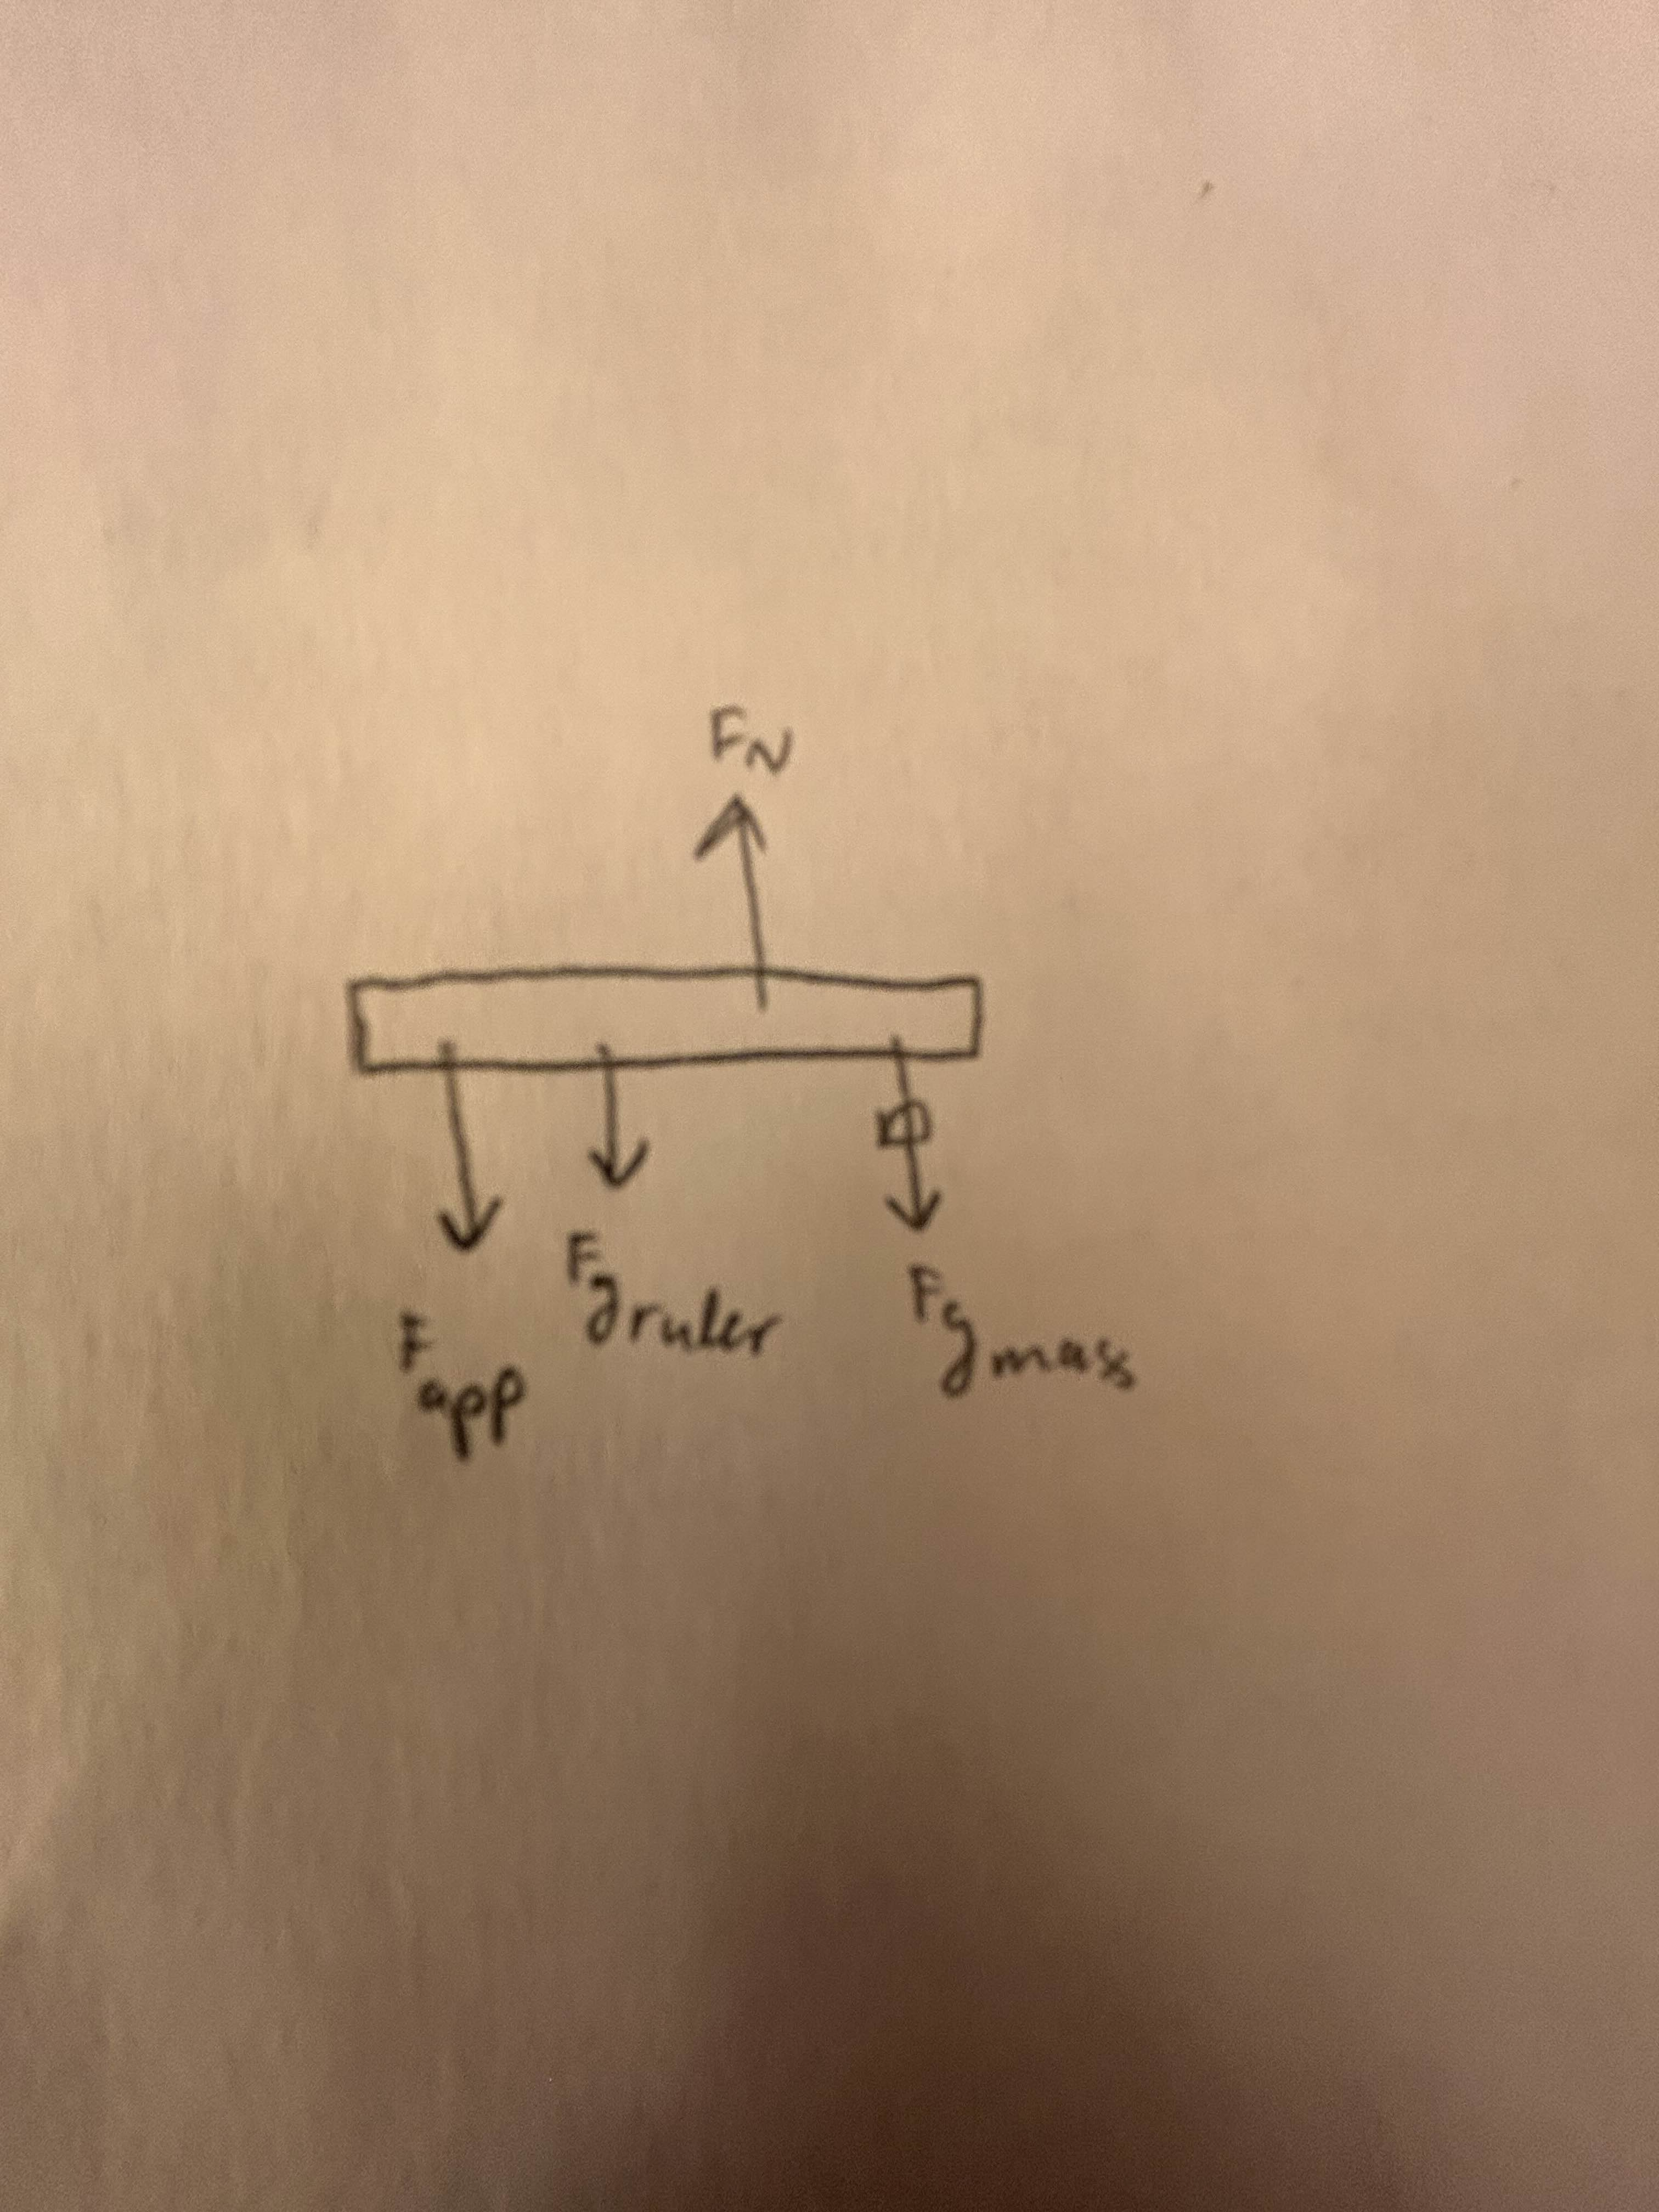
\includegraphics[height=15cm]{Lab 5.3.2.jpg}
\end{figure}
\section*{Derivation}
\[\tau = F_{app}r_{app} + F_N + {F_g}_{ruler}r_{ruler} + {F_g}_{mass}r_{mass}\]
\[F_{app} = \frac{\tau - F_N - {F_g}_{ruler}r_{ruler} - {F_g}_{mass}r_{mass}}{r_{app}}\]
Since $\tau = 0$ and $F_N = 0$ because $r_N = 0$, we obtain:
\[F_{app} = \frac{-{F_g}_{ruler}r_{ruler} - {F_g}_{mass}r_{mass}}{r_{app}}\]
\section*{Procedures}
\begin{enumerate}
    \item Place ruler on force sensor
    \item Hang mass from one end
    \item Press down on other end with second force sensor
    \item Record force from second force sensor
    \item Repeat with different positions on ruler as fulcrum
\end{enumerate}
\section*{Results}
The sign of $r$ was adjusted depending on if the force applied caused a positive (counterclockwise) rotation or negative (clockwise) rotation.
\subsection*{Constants}
These values were constant throughout the experiment.
\begin{center}
    \pgfplotstabletypeset[col sep=comma, precision=2, every head row/.style={
                before row={
                        \toprule
                    },
                after row={
                        \bottomrule
                    },
            },
        every last row/.style={
                after row=\bottomrule
            }]{Lab 5.3.2 Constants.csv}
\end{center}
\subsection*{Experimental Results}
\begin{center}
    \pgfplotstabletypeset[col sep=comma, precision=2, every head row/.style={
                before row={
                        \toprule
                    },
                after row={
                        \bottomrule
                    },
            },
        every last row/.style={
                after row=\bottomrule
            }]{Lab 5.3.2.csv}
\end{center}

Overall, our measured tension forces were lower than our calculated tension forces.
\end{document}